%%%%%%%%%%%%%%%%%%%%%%%%%%%%%%%%%%%%%%%%%%%%
\chapter{Feature Extraction}
%%%%%%%%%%%%%%%%%%%%%%%%%%%%%%%%%%%%%%%%%%%%
\begin{center}
  \begin{minipage}{0.75\textwidth}
    \begin{small}
      “Movement amongst the trees of a forest shows that the enemy is advancing.  The appearance of a number of screens in the midst of this grass means that the enemy wants to make us suspicious”.\\
      \null\hfill\emph{The Art of War, Sun Tzu}
    \end{small}
  \end{minipage}
  \vspace{0.5cm}
\end{center}

After acquiring the necessary images for calculation of a leafs' polarizance, features were extracted from the images in each color channel for texture and polarization analysis.  These features were extracted using various Python programming modules. 100 samples were extracted from each image to randomly create a training and testing set of data.  Diffuse and specular datasets were processed separately.

In order to create testing and training data, samples were extracted from each polarization image $H, V, P$ and $M$ using code found in Figure 5.1.  Each sample was extracted into three different color channels; red, green and blue.

\begin{figure}
    \begin{lstlisting}
        def extract_bgr_samples(filename, size, count):
            """
            Extract random samples from b, g, r image channels.

            Args:
                filename (str): Location to the image filename.
                size (int): The length/width of the square sample.
                count (int): The number of samples to generate.
            Returns:
                tuple: Random samples from each color channel.
            """
            img = cv2.imread(filename, 75, 1)
            samples = image.extract_patches_2d(img, (size, size), count, 1)
            cv2.imwrite('sample.png', samples[0])
            b, g, r = bgr_split(samples[0])

            return b, g, r
    \end{lstlisting}
    \caption{Extract samples from each BGR Image Channel Example Code}
    \label{fig:scattering}
\end{figure}

This type of function mentioned in Figure 5.1 can be used to extract sample patches from all three (BGR) color channels. Features can then be extracted from each of the color samples.  An example grey level histogram and image for each individual color channel through an H polarization filter can be found in Figure 5.2, 5.3 and 5.4.
\begin{figure}
    \begin{center}
        \makebox[\textwidth]{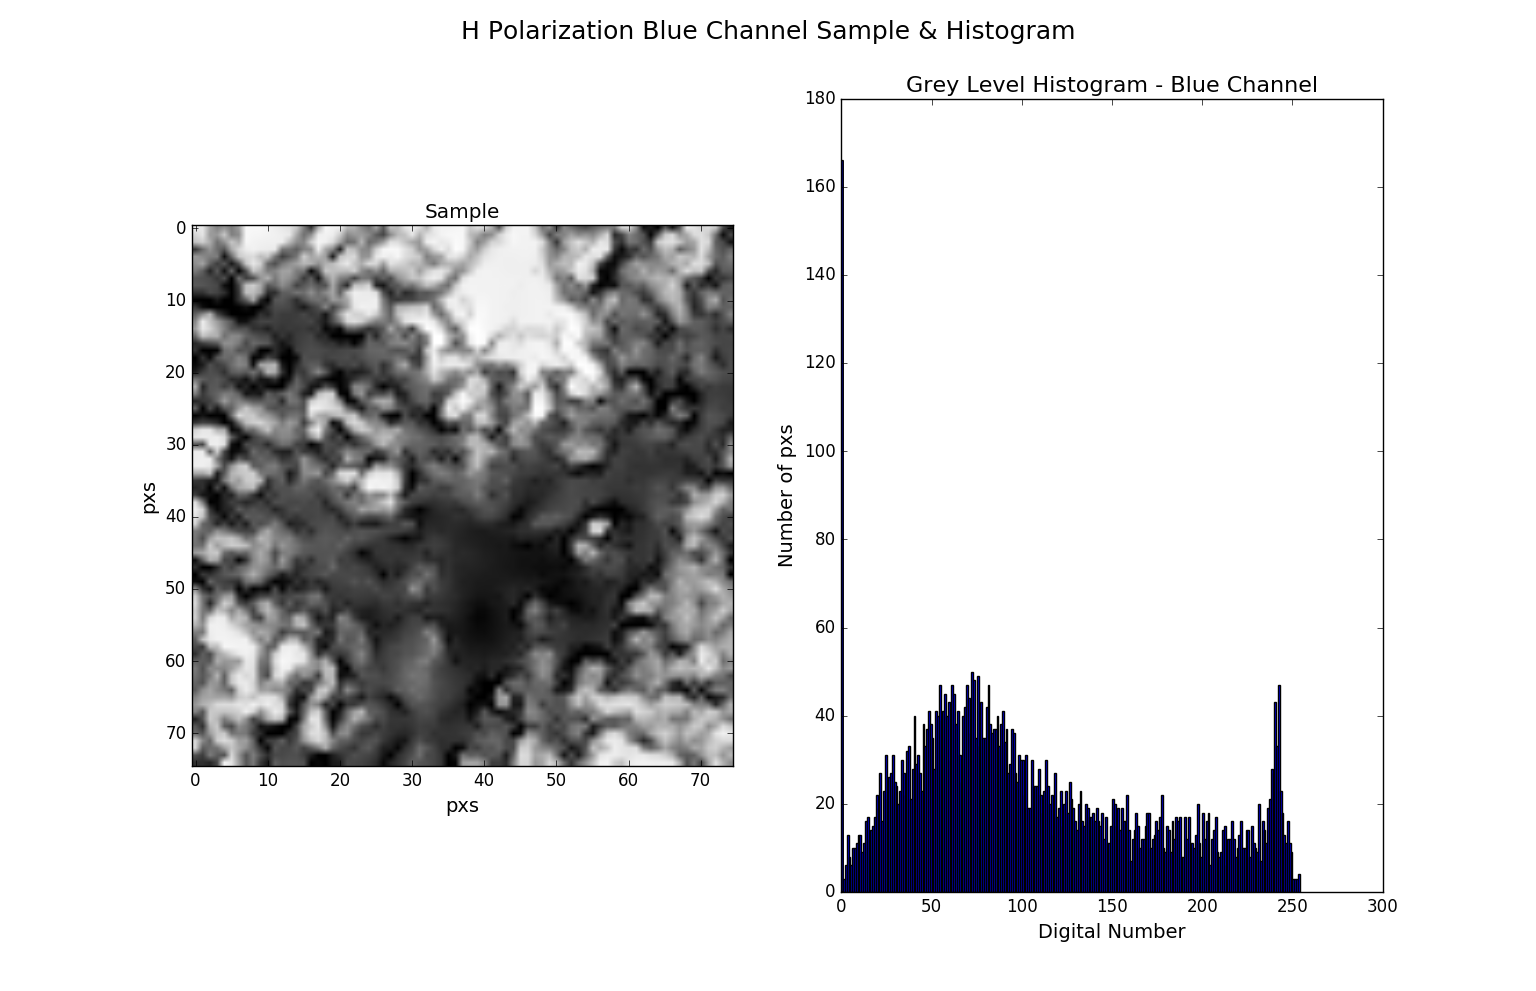
\includegraphics[scale=0.35]{/Sources/Feature_Extraction/di-H-blue-sample-hist.png}}
    \end{center}
    \caption{Devils Ivy Blue Channel H Filter Histogram}
    \label{fig:polarization}
\end{figure}
\begin{figure}
    \begin{center}
        \makebox[\textwidth]{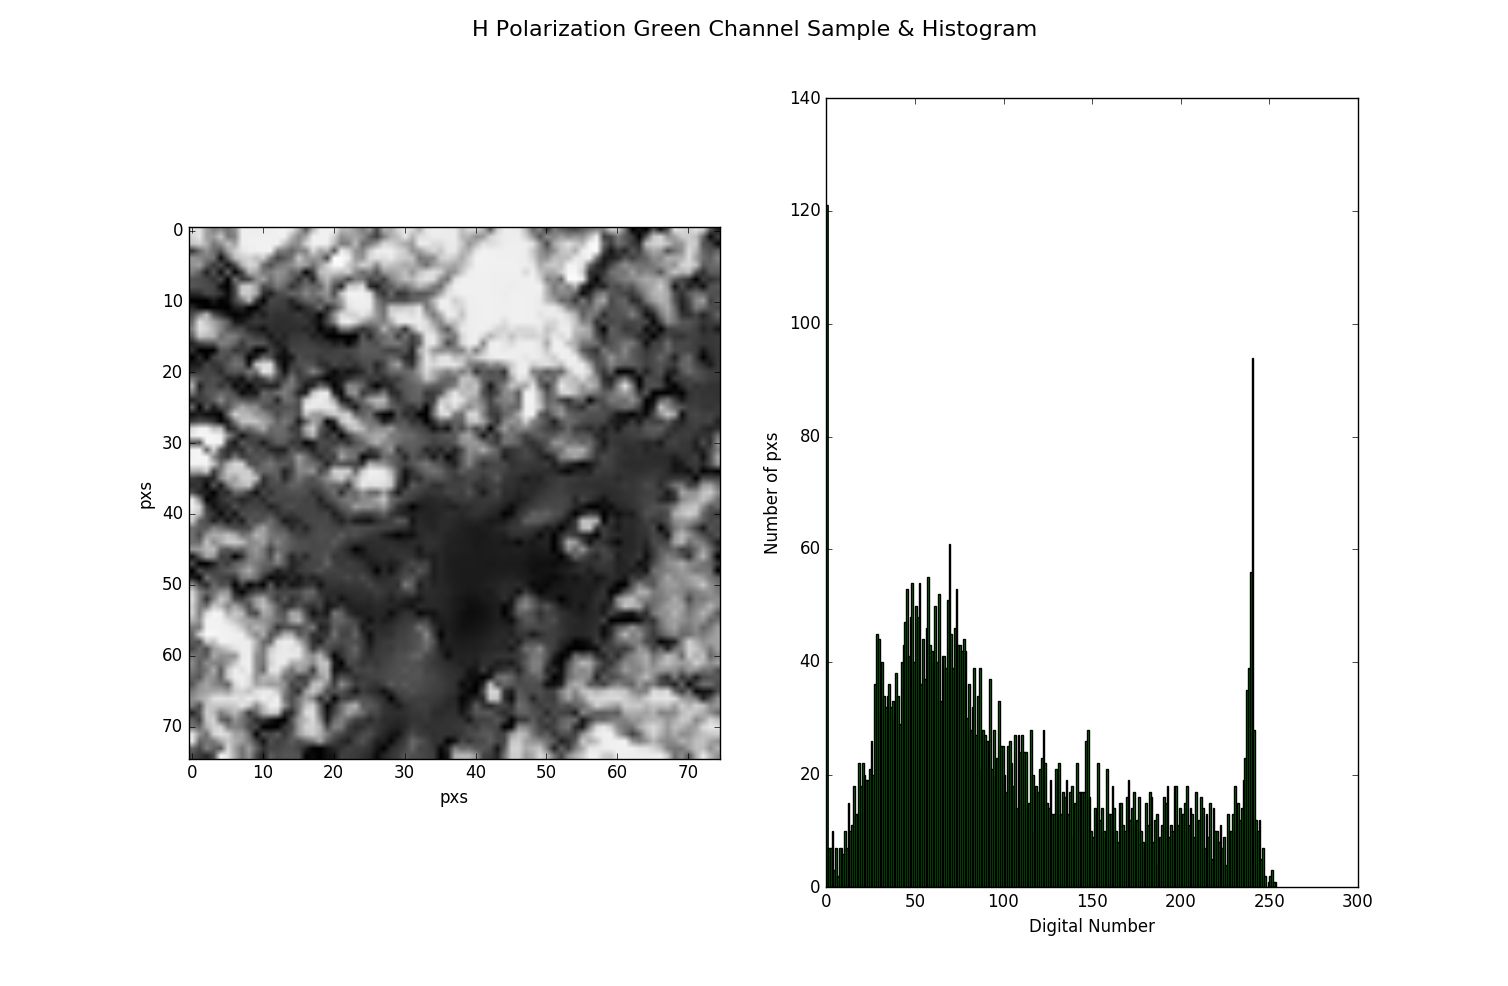
\includegraphics[scale=0.35]{/Sources/Feature_Extraction/di-H-green-sample-hist.png}}
    \end{center}
    \caption{Devils Ivy Green Channel H Filter Histogram}
    \label{fig:polarization}
\end{figure}
\begin{figure}
    \begin{center}
        \makebox[\textwidth]{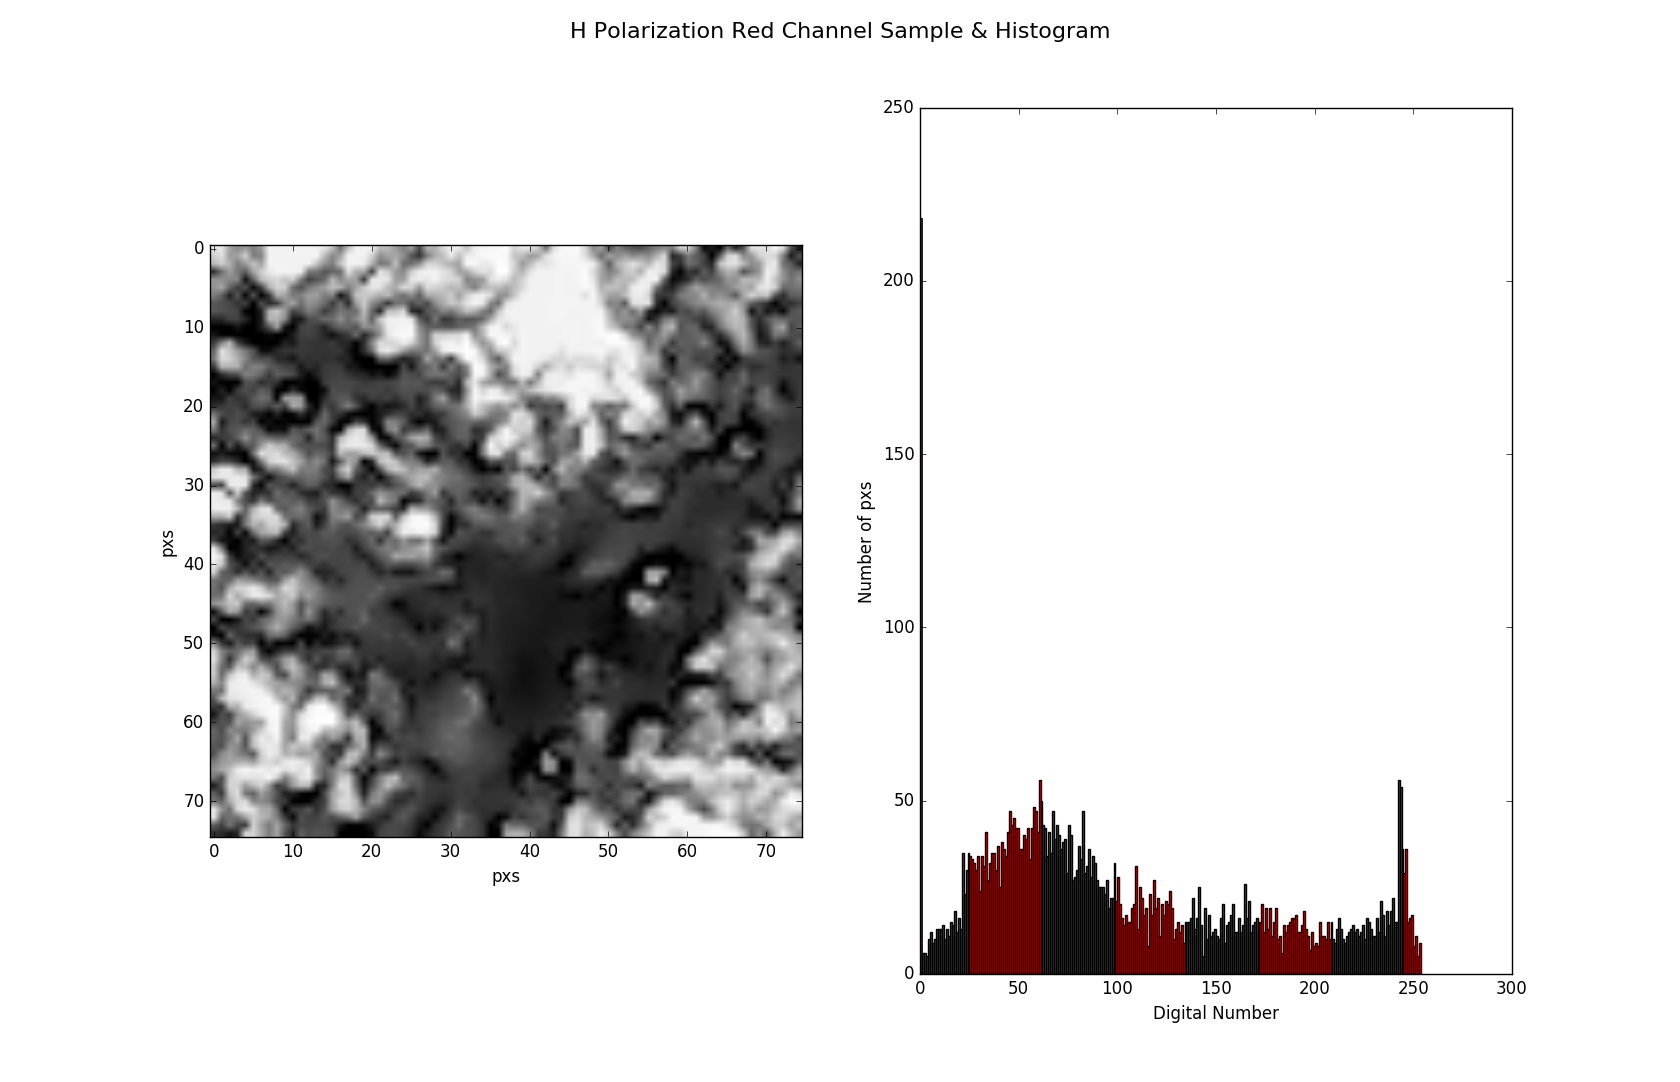
\includegraphics[scale=0.33]{/Sources/Feature_Extraction/di-H-red-sample-hist.png}}
    \end{center}
    \caption{Devils Ivy Green Channel H Filter Histogram}
    \label{fig:polarization}
\end{figure}
The corresponding V filter channels are found in Figure 5.5, 5.6 and 5.7 for a 75x75 pixel sample of Devils Ivy.
\begin{figure}
    \begin{center}
        \makebox[\textwidth]{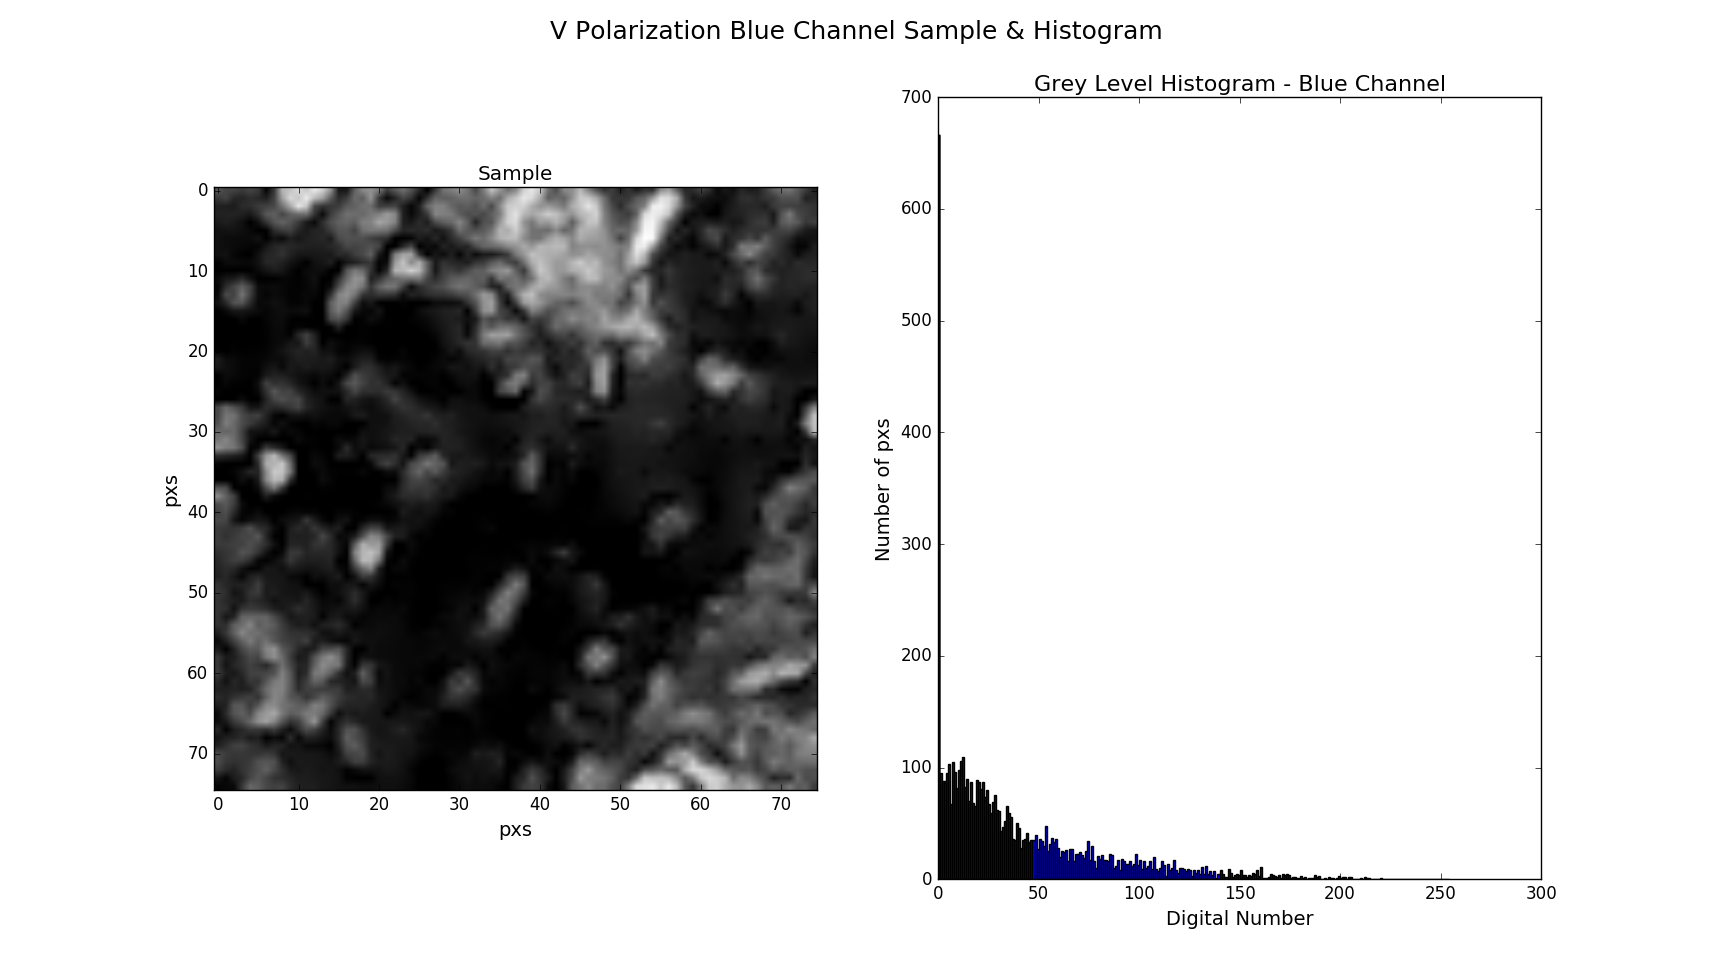
\includegraphics[scale=0.35]{/Sources/Feature_Extraction/di-V-blue-sample-hist.png}}
    \end{center}
    \caption{Devils Ivy Blue Channel V Filter Histogram}
    \label{fig:polarization}
\end{figure}
\begin{figure}
    \begin{center}
        \makebox[\textwidth]{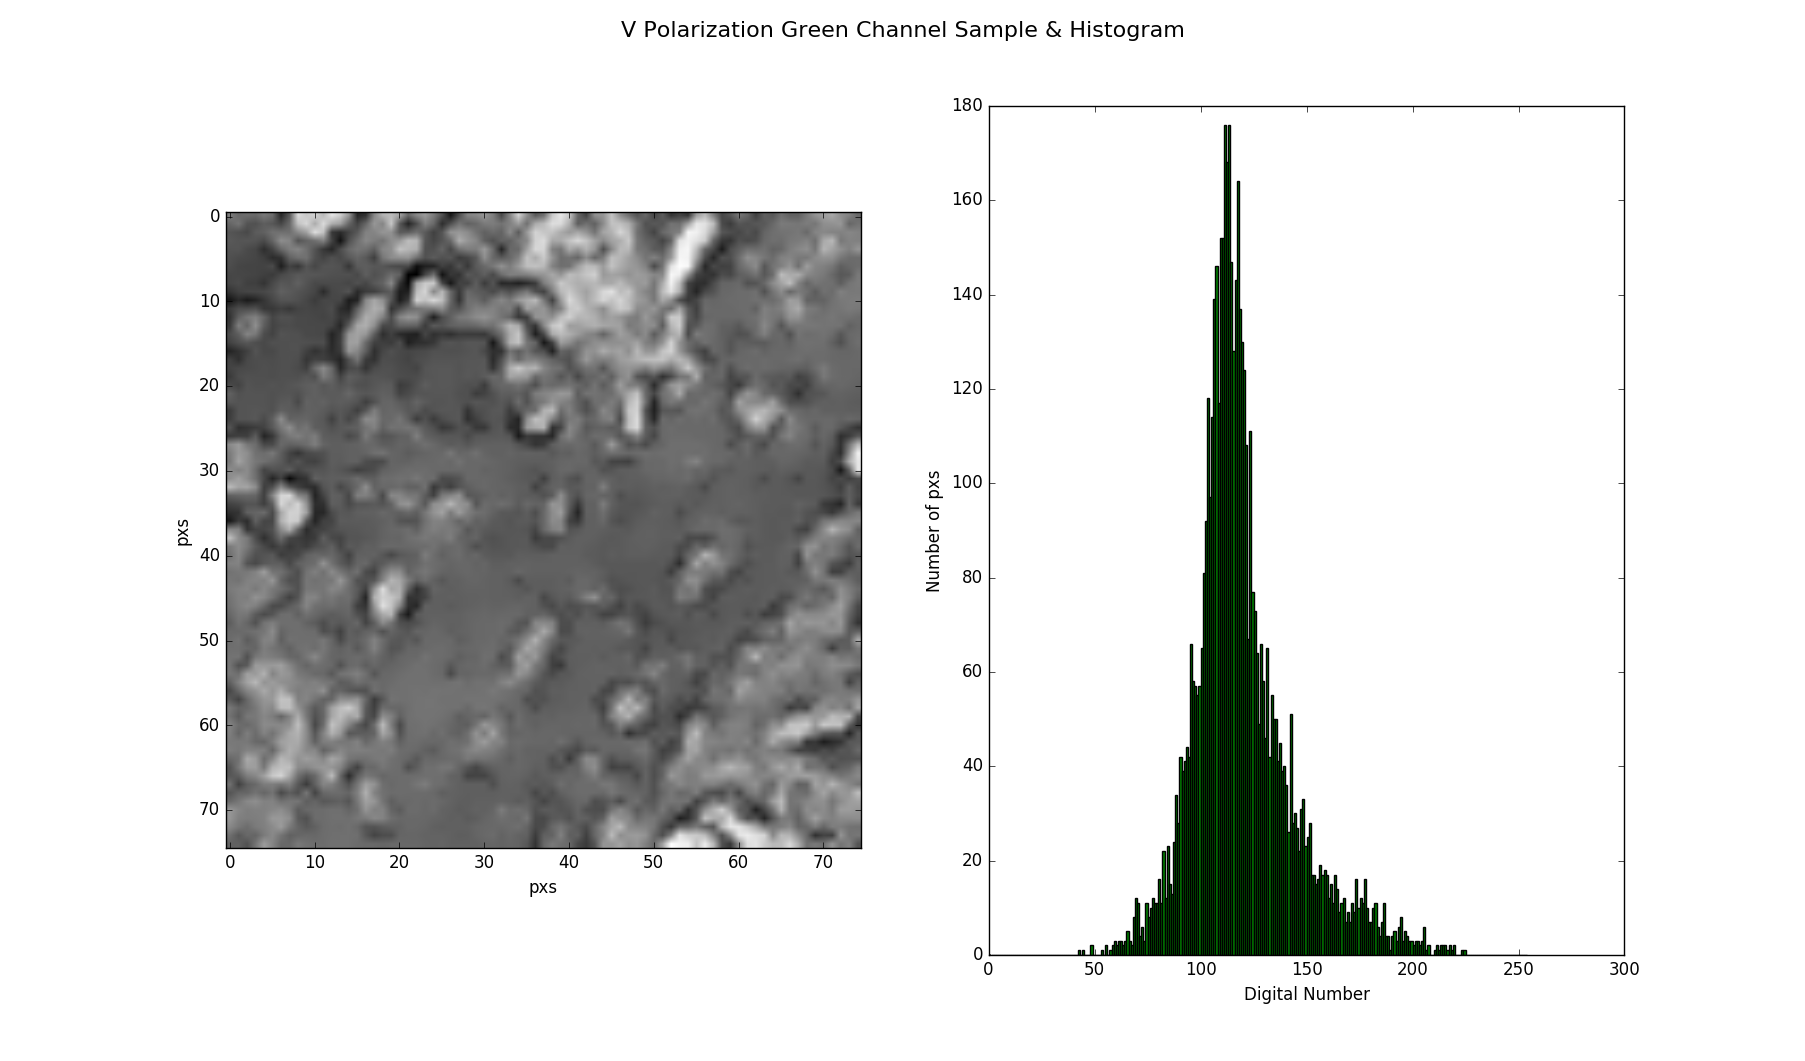
\includegraphics[scale=0.35]{/Sources/Feature_Extraction/di-V-green-sample-hist.png}}
    \end{center}
    \caption{Devils Ivy Green Channel V Filter Histogram}
    \label{fig:polarization}
\end{figure}
\begin{figure}
    \begin{center}
        \makebox[\textwidth]{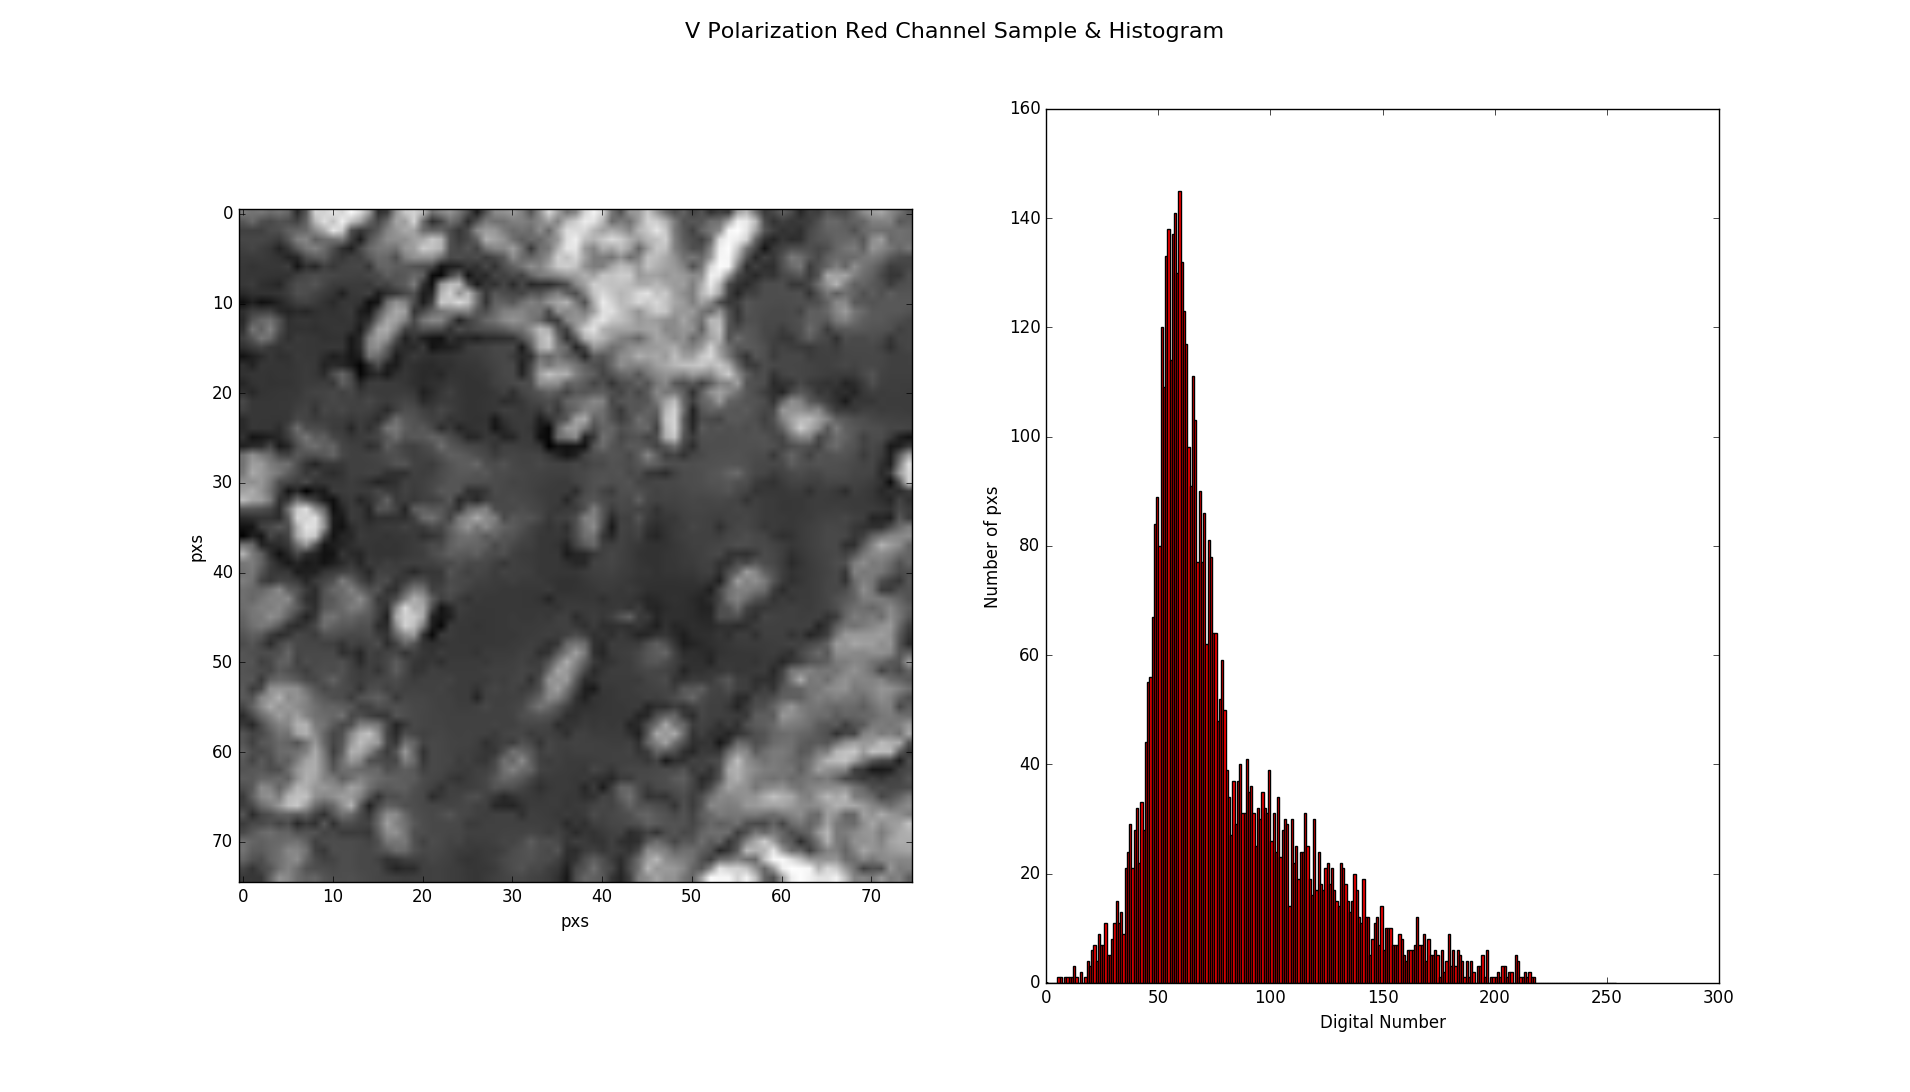
\includegraphics[scale=0.31]{/Sources/Feature_Extraction/di-V-red-sample-hist.png}}
    \end{center}
    \caption{Devils Ivy Red Channel V Filter Histogram}
    \label{fig:polarization}
\end{figure}
Each of the samples were processed using pixel based analysis, to calculate their Stokes vector as well as various GLCM metrics.  Pixels that were never illuminated were filtered out of the polarization analysis since they artificially inflated the zero mean of the produced histograms.  Polarization is not the same as light intensity and polarization can not be determined without some illumination on the target.  The Stokes vector was therefore calculated the code in Figure 5.8 where P1 and P2 represent orthogonal flux measurements through a linear polarizer.
%
\begin{figure}
    \begin{lstlisting}
        def calculate_stokes((P1, P2)):
            """
            Calulate the Stokes parameter for orthogonal images.

            Args:
                P1 (array): First polarization image.
                P2 (array): Orthogonal polarization image.
            Returns:
                array: Stokes parameters.
            """
            P1 = P1.astype(np.float32)
            P2 = P2.astype(np.float32)

            P1[np.abs(P1) < 1] = 0
            P2[np.abs(P2) < 1] = 0

            S = (P1 - P2) / (P1 + P2)

            # These represent values that have not been illuminated by the source
            # ie they are the product of masking and shadowing.
            S[~np.isfinite(S)] = 0

            return S
    \end{lstlisting}
    \caption{Example Code for Calculating the Stokes Parameters}
    \label{fig:scattering}
\end{figure}
%
These values were binned into histograms in order to reduce the dimensionality and storage requirements for the data.  These histograms were plotted using the following code in Figure 5.9.
%
\begin{figure}
    \begin{lstlisting}
        S1 = calculate_stokes((H, V))
        S2 = calculate_stokes((P, M))

        plt.title('Polarizance Paramaters')

        plt.hist(S1.ravel(), histtype='barstacked', bins=256)
        plt.hist(S2.ravel(), histtype='barstacked', bins=256)

        plt.show()
    \end{lstlisting}
    \caption{Calculate and Plot the Stokes Parameters}
    \label{fig:scattering}
\end{figure}
%
The resulting polarization histograms for a Devils Ivy sample can be found in Figure 5.10 for each corresponding BGR channel.  A false image has also been included which shows the absolute value of the S1 polarization for each channel and location on the original image.  The result of creating a false image out of the a polarization matrix, allows for a visualization for how polarization is resulting from specific surface and subsurface features.
\begin{figure}
    \begin{center}
        \makebox[\textwidth]{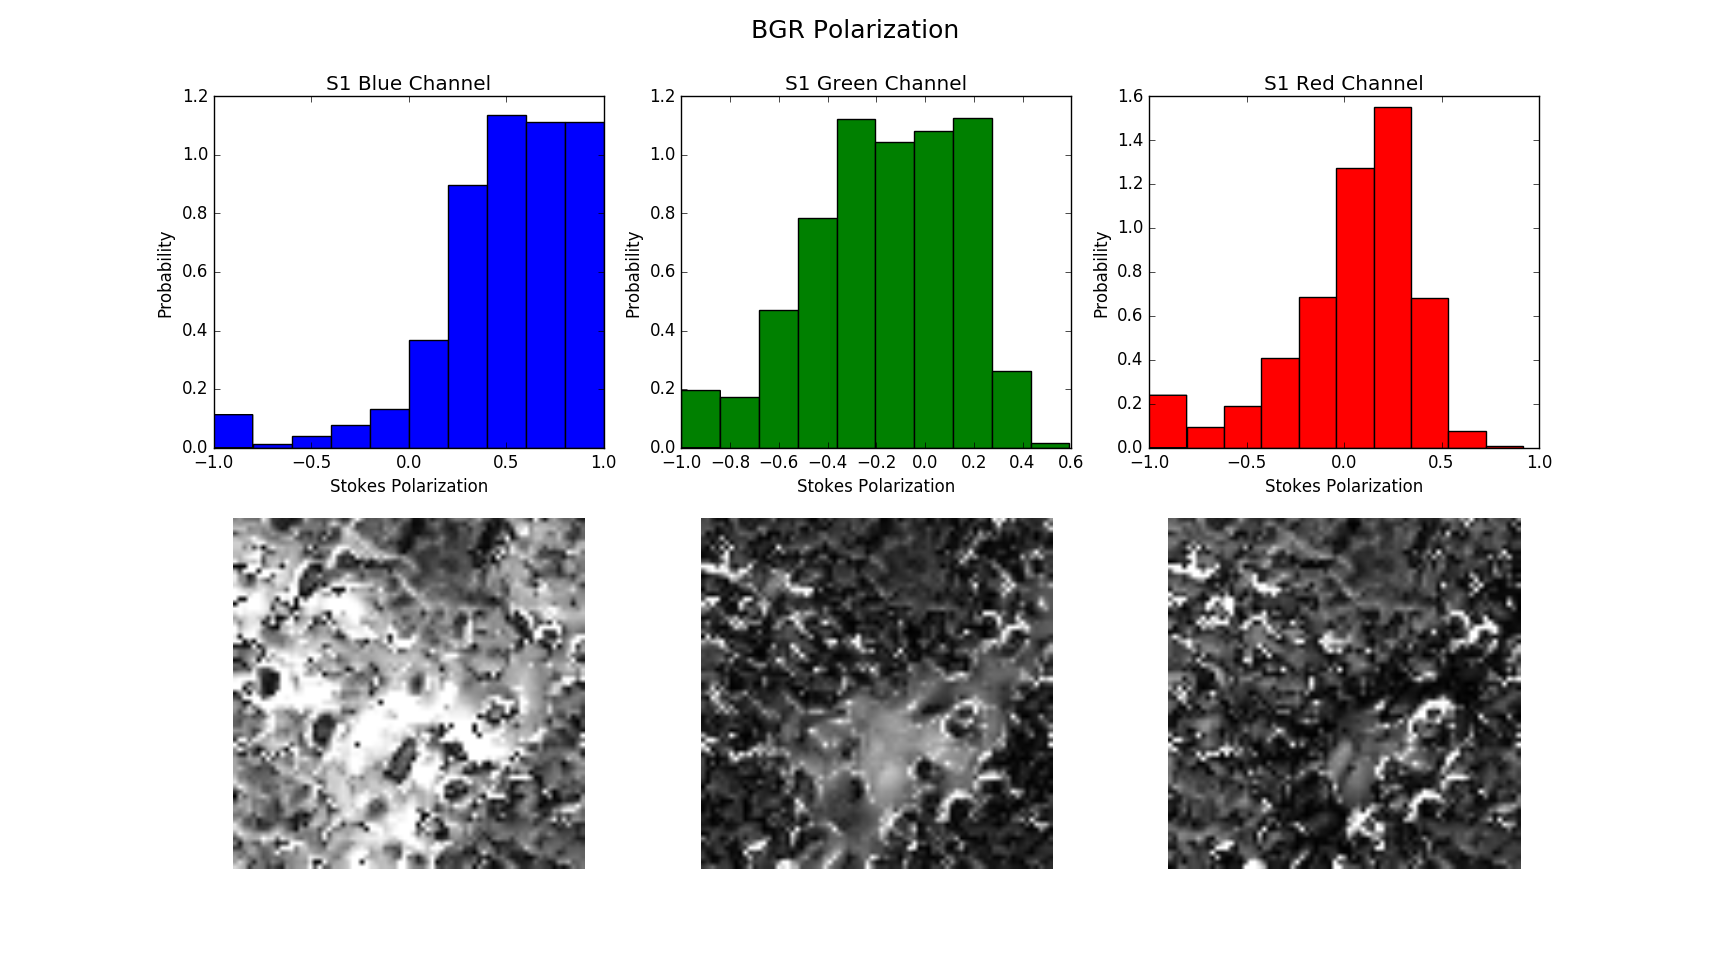
\includegraphics[scale=0.35]{/Sources/Feature_Extraction/di-bgr-s1-v2.png}}
    \end{center}
    \caption{BGR Histograms for Devils Ivy Sample S1 Polarization Parameter}
    \label{fig:polarization}
\end{figure}
Window-based GLCM texture analysis was similarly performed on each of the extracted samples.  The dissimilarity, correlation, contrast and entropy were calculated for each GLCM.  The window size for GLCM was manually optimized by testing clustering effects for 5px, 9px, 25px, 55px, 75px, and 95px window sizes.  A window size of 75 pixels was found to be ideal for this experimental design.

In addition to performing a polarization based analysis on each color channel of the extracted samples, a GLCM texture analysis was also performed.  The dissimilarity, contrast, correlation and energy were calculated for each sample window.  The following code was used for these calculations,
\begin{figure}
    \begin{lstlisting}
        def extract_texture(samples):
            """
            Generate GLCM based texture features for a given color channel.

            Args:
                samples (array): Array containing each image sample.  Each sample is a
                    matrix of pixel intensities for a single color channel.
            Returns:
                array: Texture features extracted for an individual color channel.
            """
            texture = []
            for sample in samples:
                try:
                    # Calculate texture features for a given sample
                    relationships = [0, np.pi/4, np.pi/2, 3*np.pi/4]
                    glcm = greycomatrix(sample, [1], relationships, 256, symmetric=True, normed=True)
                    metrics = ['dissimilarity', 'contrast', 'correlation', 'energy']
                    diss, contrast, corr, energy = [greycoprops(glcm, metric)[0, 0] for metric in metrics]

                    texture.append([diss, contrast, corr, energy])
                except ValueError:
                    print "Error in extracting the texture features"

            return np.array(texture)
    \end{lstlisting}
    \caption{noobee code for Jones Vectors}
    \label{fig:scattering}
\end{figure}
The metrics derived from the GLCM matrix can be plotted in various scatterplots as demonstrated in the Results chapter and Appendix. Data was exported to .csv files for future processing and analysis in Support Vector Machine classification and linear regression.
Pixel-based, histogram counts and GLCM derived, window-based metrics were combined to form feature vector sets in the classification and regressions given in Chapter 7.
